\section{Die Simulation}
\begin{figure}
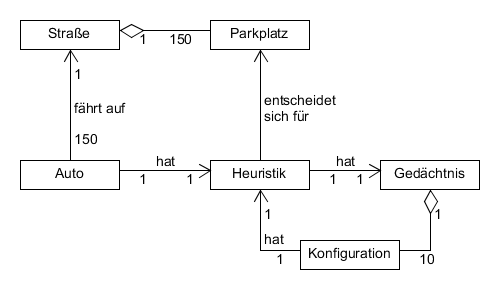
\includegraphics[width=0.5\textwidth]{uml/simOverview.png}
\caption{Strukturelle Übersicht der Simulation}\label{fig_simOver}
\end{figure}
\subsection{Aufbau der Simulation}
Um die Konfigurationen für die Heuristiken zu lernen wird die Parkplatzsuche simuliert. Da in dieser Arbeit mehrere Fragen beantwortet werden sollen, sind auch mehrere Simulationen mit unterschiedlichen Randbedingungen notwendig. Der Grundlegende Aufbau jeder Simulation ist jedoch gleich und in Abbildung \ref{fig_simOver} dargestellt. 

\subsubsection{Unterschiede zu Hutchinson et al}

\subsection{Wahl der Parameter}
